\centerline{\Large \textbf{Supplementary material (not part of the paper)}}


%%%%%%%%%%%%%%%%%%%%%%%%%%%%%%%%%%%%%%%%%%%%%%%%%%%%%%%%%%%%%%%%
\section{Details for the MSGD training approach}\label{appen:MSGDtraining}

The MSGD method estimates the penalty function $\mathcal{O}(\theta)$, which is typically unknown, through small samples of the hedging error called batches. Let $\mathbb{B}_{j}=\{ \xi_{T,i}^{\tilde{\delta}_{\theta_{j}}} \}_{i=1}^{N_{\mbox{\scriptsize{batch}}}}$ be the $j$-th batch where $N_{\mbox{\scriptsize{batch}}}$ is the batch size and $\xi_{T,i}^{\tilde{\delta}_{\theta_{j}}}$ denotes the hedging error of the $i$-th path in the $j$-th batch defined as
$$\xi_{T,i}^{\tilde{\delta}_{\theta_{j}}} = \Psi(S_{T,(j-1)N_{\mbox{\scriptsize{batch}}}+i}) - V_{T,i}^{\tilde{\delta}_{\theta_{j}}} \quad \mbox{for} \quad i\in\{1,\dots,N_{\mbox{\scriptsize{batch}}}\}, \, j\in\{1,...N \},$$
where $S_{T,(j-1)N_{\mbox{\scriptsize{batch}}}+i}$ is the price of the underlying asset at time $T$ in the ($(j-1)N_{\mbox{\scriptsize{batch}}}+i$)-th simulated path, $V_{T,i}^{\tilde{\delta}_{\theta_{j}}}$ is the terminal value of the hedging strategy for that path when $\theta = \theta_{j}$ and the simulated states are $X_{i}$. 

The penalty function estimation for the batch $\mathbb{B}$ is
\begin{align*}
    \Hat{C}^{\left(\mbox{\scriptsize{MSE}}\right)}(\theta_{j},\mathbb{B}_{j})&=\frac{1}{N_{\mbox{\scriptsize{batch}}}}\sum_{i=1}^{N_{\mbox{\scriptsize{batch}}}}\left(\xi_{T,i}^{\tilde{\delta}_{\theta_{j}}}\right)^{2}\, \mbox{,}\\
    \Hat{C}^{\left(\mbox{\scriptsize{SMSE}}\right)}(\theta_{j},\mathbb{B}_{j})&=\frac{1}{N_{\mbox{\scriptsize{batch}}}}\sum_{i=1}^{N_{\mbox{\scriptsize{batch}}}}\left(\xi_{T,i}^{\tilde{\delta}_{\theta_{j}}}\right)^{2}\mathbbm{1}_{\left\{\xi_{T,i}^{\tilde{\delta}_{\theta_{j}}}\geq 0\right\}}\, \mbox{,}\\
    \Hat{C}^{\left(\mbox{\scriptsize{CVaR}}\right)}(\theta_{j},\mathbb{B}_{j})&= \widehat{\mbox{VaR}}_{\alpha}(\mathbb{B}_{j})+\frac{1}{(1-\alpha)N_{\mbox{\scriptsize{batch}}}}\sum_{i=1}^{N_{\mbox{\scriptsize{batch}}}}\max\left( \xi_{T,i}^{\tilde{\delta}_{\theta_{j}}}-\widehat{\mbox{VaR}}_{\alpha}(\mathbb{B}_{j}),0 \right)\, \mbox{,}
\end{align*}

where $\widehat{\mbox{VaR}}_{\alpha}(\mathbb{B}_{j})=\xi_{T,\lceil \alpha \cdot N_{\mbox{\scriptsize{batch}}} \rceil}^{\tilde{\delta}_{\theta_{j}}}$ is the estimation of the VaR obtained from the ordered sample $\{ \xi_{T,[i]}^{\tilde{\delta}_{\theta_{j}}} \}_{i=1}^{N_{\mbox{\scriptsize{batch}}}}$ and $\lceil \cdot \rceil$ is the ceiling function. These empirical approximations are used to estimate the gradient of the penalty function required in Equation \eqref{updatingrule}.\footnote{In particular, the gradient of these estimations has analytical expressions for FFNN, LSTM networks and thus for RNN-FNN networks. Details about gradient of the empirical objective function are provided in \cite{goodfellow2016deep}.} %The gradient estimate $\nabla_{\theta}\hat{\mathcal{O}}$ is calculated with automatic differentiation packages.

The selection of batch size plays a key role in the MSGD training approach as we empirically measure tail risk. A larger batch size provides a more accurate gradient estimate by averaging gradients computed over more simulated paths, thereby promoting stable convergence during training. However, large batch sizes may introduce certain disadvantages such as increased memory requirements, slower convergence, and potential generalization issues. We adopt the batch size used in \cite{carbonneau2021deep} ($N_{\mbox{\scriptsize{batch}}}=1,\!000$), which achieves a good balance between accuracy and convergence.


%%%%%%%%%%%%%%%%%%%%%%%%%%%%%%%%%%%%%%%%%%%%%%%%%%%%%%%%%%%%%%
\section{Joint Implied Volatility and Return model}\label{appen:JIVR}

\subsection{Daily implied volatility surface}\label{subappen:IVsurface}

The functional representation of the IV surface model introduced by \cite{Frnacois2022} is
\begin{align}
     & \sigma (M_{t},\tau_{t},\beta_{t}) =  \underbrace{\beta_{t,1}}_{f_{1}\mbox{: \scriptsize{Long-term ATM IV}}} +  \beta_{t,2}\underbrace{e^{-\sqrt{\tau_{t} /T_{conv}}}}_{f_{2}\mbox{: \scriptsize{Time-to-maturity slope}}} + \beta_{t,3}\underbrace{\left( M_{t}\mathbbm{1}_{\{ M_{t}\geq 0 \}} + \frac{e^{2M_{t}}-1}{e^{2M_{t}}+1}\mathbbm{1}_{\{M_{t}< 0\}} \right)}_{f_{3}\mbox{: \scriptsize{Moneyness slope}}} \nonumber\\
     & + \beta_{t,4}\underbrace{\left( 1-e^{-M_{t}^{2}} \right)\mbox{log}(\tau_{t}/T_{max})}_{f_{4}\mbox{: \scriptsize{Smile attenuation}}}+\beta_{t,5}\underbrace{\left( 1-e^{(3M_{t})^{3}} \right)\mbox{log}(\tau_{t}/T_{max})\mathbbm{1}_{\{M_{t}< 0\}}}_{f_{5}\mbox{: \scriptsize{Smirk}}}\, , \quad \tau_{t} \in [T_{min},T_{max}] 
     \label{full_5factormodel}
\end{align}

where $T_{max}$ is set to 5 years, $T_{min}=6/252$ and $T_{conv}=0.25$. As in \cite{dumas1998implied},  a minimum threshold of 0.01 is applied to the volatility surface to prevent negative values.

\subsection{Joint Implied Volatility and Return}\label{subappen:JIVR_timeseries}

The JIVR model proposed by \cite{Frnacois2023} has 6 components, one for the underlying asset excess returns and the other 5 for fluctuations of the IV surface coefficients. The S\&P 500 excess return follows:
 \begin{align}
     R_{t+1} & = \xi_{t+1}-\psi(\sqrt{h_{t+1,R}\Delta}) + \sqrt{h_{t+1,R}\Delta}\epsilon_{t+1,R}, \nonumber\\
     h_{t+1,R} & = Y_{t}+\kappa_{R}(h_{t,R}-Y_{t})+a_{R}h_{t,R}(\epsilon_{t,R}^{2}-1-2\gamma_{R}\epsilon_{t,R}), \label{return}\\
     Y_{t} &= \left(\omega_{R}\, \sigma \left(0,\frac{1}{12},\beta_{t}\right)\right)^2, \nonumber
     \label{returnseries}
 \end{align}
where the equity risk premium is
\begin{equation}
    \xi_{t+1}=\psi(-\lambda\sqrt{h_{t+1,R}\Delta})- \psi((1-\lambda)\sqrt{h_{t+1,R}\Delta}) + \psi(\sqrt{h_{t+1,R}\Delta}),
\end{equation}
the process $\{\epsilon_{t,R}\}^T_{t=0}$ is a sequence of iid standardized NIG random variables with parameters $\zeta_{R}$ and $\varphi_{R}$,\footnote{The standard NIG random variable $\epsilon$ follows the probability density function with parameters $\zeta$ and $\varphi$: $$f(x)=\frac{B_{1}\left( \sqrt{\frac{\varphi^{6}}{\varphi^{2}+\zeta^{2}}+(\varphi^{2}+\zeta^{2})\left(x+ \frac{\varphi^{2}\zeta}{\varphi^{2}+\zeta^{2}} \right)^{2}} \right)}{\pi\sqrt{\frac{1}{\varphi^{2}+\zeta^{2}}+\frac{\varphi^{2}+\zeta^{2}}{\varphi^{6}}\left(x+ \frac{\varphi^{2}\zeta}{\varphi^{2}+\zeta^{2}} \right)^{2}} } e^{\left( \frac{\varphi^{4}}{\varphi^{2}+\zeta^{2}}+\zeta\left(x+ \frac{\varphi^{2}\zeta}{\varphi^{2}+\zeta^{2}} \right) \right),}$$ where $B_{1}(\cdot)$ denotes the modified Bessel function of the second kind with index 1. The common $(\alpha, \beta, \delta, \mu)$-specification can be obtained by replacing $\beta$ and $\gamma$ ($\gamma = \sqrt{\alpha^2-\beta^2}$), with $\zeta$ and $\varphi$, respectively, and imposing a null mean and unit variance to express $\delta$ and $\mu$ interms of $\alpha$, $\beta$.} 
and $\psi$ is their cumulant generating function.\footnote{For $-\sqrt{\zeta^{2}+\varphi^{2}}-\zeta<z<\sqrt{\zeta^{2}+\varphi^{2}}-\zeta$, the cumulant generating function is given by 
$$\psi(z)=\frac{\varphi^{2}}{\varphi^{2}+\zeta^{2}}\left( -\zeta z+\varphi^{2}-\varphi\sqrt{\varphi^{2}+\zeta^{2}-(\varphi+\zeta)^{2}} \right).$$}
Parameters of the excess return component of the model are thus $\Theta_{R} = (\lambda,\kappa_{R},\gamma_{R},a_{R},\omega_{R},\zeta_{R},\varphi_{R})$. 

The evolution of the long-term factor $(\beta_{1})$ is
\begin{align}
     \beta_{t+1,1}&= \alpha_{1}+\sum_{i=1}^{5}\theta_{1,j}\beta_{t,j}+\sqrt{h_{t+1,1}\Delta}\epsilon_{t+1,1}, \nonumber\\
     h_{t+1,1} &= U_{t}+\kappa_{1}(h_{t,1}-U_{t})+a_{1}h_{t,1}(\epsilon_{t,1}^{2}-1-2\gamma_{1}\epsilon_{t,1}), \label{beta1series}\\
     U_{t} &= \left(\omega_{1}\cdot \sigma\left(0,\frac{1}{12},\beta_{t}\right)\right)^2. \nonumber
 \end{align}

For the other 4 coefficients, $i\in\{2,3,4,5 \}$, the time evolution satisfies
\begin{align}
    \beta_{t+1,i} &= \alpha_{i}+\sum_{j=1}^{5}\theta_{i,j}\beta_{t,j}+\nu\beta_{t-1,2}\mathds{1}_{\{i=2\}}+\sqrt{h_{t+1,i}\Delta}\epsilon_{t+1,i}, \nonumber\\
    h_{t+1,i} &= \sigma_{i}^{2}+\kappa_{i}(h_{t,i}-\sigma_{i}^{2})+a_{i}h_{t,i}(\epsilon_{t,i}^{2}-1-2\gamma_{i}\epsilon_{t,i}),
    \label{restofbetas}
\end{align}

where $\{\epsilon_{t,i} \}_{i=1}^{5}$ are time-independent standardized NIG random variables with parameters $\{ (\zeta_{i},\varphi_{i}) \}_{i=1}^{5}$, respectively. Parameters are $\{\omega_{1},\nu, \Theta_{1}, \Theta_{2}, \Theta_{3}, \Theta_{4}, \Theta_{5}\}$ with $\Theta_{i} = (\alpha_{i},\{\theta_{i,1}\}_{i=1}^{5},\sigma_{i},\kappa_{i},a_{i},\gamma_{i},\zeta_{i},\varphi_{i})\}_{i=1}^{5}$.

The JIVR model also imposes a dependence structure on contemporaneous innovations $\epsilon_{t} = (\epsilon_{t,R},\epsilon_{t,1},...,\epsilon_{t,5})$ through a Gaussian copula parameterized in terms of a covariance matrix $\Sigma$ of dimension ${6\times 6}$. 

Estimates of all JIVR model parameters are taken from Table 5 and Table 6 of \cite{Frnacois2023}. 


\section{JIVR Model parameters}

\begin{table}[H]
\centering
\renewcommand{\arraystretch}{1.5}
\caption{Estimated Gaussian copula parameters}
\begin{tabular}{lrrrrrr}
\toprule
 & $\epsilon_{t,R}$ & $\epsilon_{t,1}$ & $\epsilon_{t,2}$ & $\epsilon_{t,3}$ & $\epsilon_{t,4}$ & $\epsilon_{t,5}$ \\
\midrule
$\epsilon_{t,R}$ & 1.000 &  &  &  & &  \\
$\epsilon_{t,1}$ & -0.550 & 1.000 &  &  &  &  \\
$\epsilon_{t,2}$ & -0.690 & 0.140 & 1.000 &  & &  \\
$\epsilon_{t,3}$ & 0.030 & -0.030 & -0.0100 & 1.000 &  &  \\
$\epsilon_{t,4}$ & -0.220 & 0.250 & 0.120 & 0.280 & 1.000 &  \\
$\epsilon_{t,5}$ & -0.340 & 0.170 & 0.370 & 0.130 & -0.050 & 1.000 \\
\bottomrule
\end{tabular}
\end{table}

\begin{table}[H]
\centering
\renewcommand{\arraystretch}{1.5}
\caption{ JIVR model parameter estimates }
\begin{tabular}{lrrrrrrr}
\toprule
Parameter  & $\beta_1$ & $\beta_2$ & $\beta_3$ & $\beta_4$ & $\beta_5$ & & S\&P500 \\
\cline{1-6}\cline{8-8}
$\alpha$ & 0.000899 & 0.008400 & 0.000770 & -0.001393 & 0.000657 & $\lambda$ & 2.711279 \\
$\theta_1$ & 0.996290 & -0.013869 &  & 0.002841 &  &  &\\
$\theta_2$ & 0.003669 & 0.877813 & 0.001300 &  &  &  &\\
$\theta_3$ &  & -0.032640 & 0.997071 & 0.003722 & -0.004198 &  &\\
$\theta_4$ &  &  &  & 0.980269 &  &  &\\
$\theta_5$ &  & -0.047789 &  &  & 0.986019 &  &\\
$\nu$ &  & 0.089445 &  &  &  &  &\\
$\sigma\sqrt{252}$ &  & 0.380279 & 0.052198 & 0.048641 & 0.051536 &  &\\
$\omega$ & 0.267589 &  &  &  &  & & 0.977291 \\
$\kappa$ & 0.838220 & 0.965751 & 0.974251 & 0.945377 & 0.980844 & & 0.888977 \\
$a$ & 0.134152 & 0.098272 & 0.092646 & 0.102201 & 0.100502 & & 0.056087 \\
$\gamma$ & -0.111813 & -1.482862 & 0.096766 & 0.060558 & -0.102996 & & 2.507796 \\
$\zeta$ & 0.143760 & 0.852943 & 0.029109 & -0.159051 & 0.092664 & & -0.641306 \\
$\varphi$ & 1.351070 & 1.538928 & 2.284780 & 1.449977 & 1.428477 & & 2.039669 \\
\bottomrule
\end{tabular}
\end{table}

%%%%%%%%%%%%%%%%%%%%%%%%%%%%%%%%%%


\section{Network fine-tuning}

\subsection{Bounded strategies - leverage constraint}\label{se:Bounded strategies - leverage constraint}

This section presents a comparison of the hedging performance of RL agents trained under the full state space considering the CVaR$_{95\%}$ as penalty function. The comparison is conducted considering two RL agents: (i) RL-CVaR$_{95\%}$-LC, agent subject to a leverage constraint  equivalent to the initial value of the underlying asset, set at $B=100$, and (ii) RL-CVaR$_{95\%}$, agent operating without leverage constraints. This comparison evaluates the estimated values of all penalty functions and the average Profit and Loss (Avg P\&L). This analysis aims to elucidate the impact of boundary conditions on RL agent behavior and performance when hedging of a European ATM call option with a maturity of $N=63$ days in the absence of transaction costs, i.e., $\kappa = 0\%$).

\autoref{table:cash_constraint} outlines that the agent without a leverage constraint shows more profitable strategies; however, it also leads to very large losses. For instance, out-of-sample CVaR$_{99\%}$ and SMSE metrics exhibit higher values for this agent, compared to its counterpart with a leverage constraint. 

\begin{table}[H]
\centering
\renewcommand{\arraystretch}{1.5}
\caption{RNN-FNN hedging error statistics of a short position in a ATM call option with maturity of 63 days.}
\begin{tabular}{p{2.5cm} >{\centering\arraybackslash}p{3.2cm} >{\centering\arraybackslash}p{3.2cm}}
\hline
Function & RL-CVaR$_{95\%}$-LC & RL-CVaR$_{95\%}$ \\
\hline
Avg P\&L & 0.440 &   {\bfseries 0.715} \\
CVaR$_{95\%}$ & 1.294 &   {\bfseries 1.242} \\
CVaR$_{99\%}$ & {\bfseries 2.502} &   2.622 \\
MSE & {\bfseries 1.205} &   14.650 \\
SMSE & {\bfseries 0.241} &   0.327 \\
\hline
\end{tabular}
\label{table:cash_constraint}
\begin{tablenotes}
\item \footnotesize Results are computed using 100,000 out-of-sample paths in the absence of transaction costs ($\kappa = 0\%$). Agents are trained under the full state space $(V_{t}^{\delta},\delta_{t},\tau_{t},S_{t},\{\beta_{t,i} \}^5_{i=1}, h_{t,R}, \{ h_{t,i}\}^5_{i=1})$ according to the conditions outlined in Section \ref{subsub:network_architecture}. The average option price is \$3.89 with a standard deviation of \$1.29. RL-CVaR$_{95\%}$-LC denotes the RL agent trained with a leverage constraint, while RL-CVaR$_{95\%}$ refers to the agent without it. Best performances are highlighted in bold. 
\end{tablenotes}
\end{table}

Moreover, our numerical experiments demonstrate that the agent without leverage constraints learns doubling strategies, which are incompatible with sound risk management practices. For instance, \autoref{fig:Martingale_startegies} illustrates such behavior through three panels associated with the hedging process of a deep OTM path (first panel).\footnote{For the purpose of this experiment, a deep OTM path refers to the trajectory of the underlying asset that keeps the option significantly out-of-the-money.} We observe that the agent, without a leverage constraint, tends to increase its position in the underlying (third panel) when a loss in the portfolio value is observed (second panel), aiming to recover the loss over the long run with doubling strategies. Conversely, agents trained with a leverage constraint control their position in the underlying asset, resulting in the learning of different and less risky strategies. 

\begin{figure}[h]\centering
\caption{Doubling strategy dynamics for a short position in a ATM call option with a maturity of 63 days.}

\includegraphics[width=17cm]{martingale.pdf}
\label{fig:Martingale_startegies}
\begin{tablenotes}
\item \footnotesize Results are obtained using a deep OTM path in the absence of transaction costs ($\kappa = 0\%$), with agents trained according to the conditions outlined in Section \ref{subsub:network_architecture}. The training encompasses the full state space and utilizes CVaR$_{95\%}$ as a penalty function. The agent referred to as "Agent with cash constraint" incorporates a leverage constraint of $B=100$, whereas the agent labeled "Agent without cash constraint" does not.
\end{tablenotes}
\end{figure}

%%%%%%%%%%%%%%%%%%%%%%%%%%%%%%%%%%%%%%%%%%%%%%%

\subsection{Network architecture selection}\label{appen:architecture_selection}

In this section, we investigate the superiority of the RNN-FNN architecture compared to conventional architectures introduced in deep hedging literature, such as the FFNN and the LSTM architectures. In line with our previous experiments, we consider four penalty functions to train the agents under the full state space: CVaR$_{95\%}$, CVaR$_{99\%}$, MSE, and SMSE. Again, our experiment focuses on hedging a short position of a European ATM call option with a maturity of $N=63$ days, assuming no transaction costs.

The superiority of the RNN-FNN over the LSTM and the FFNN is evaluated based on the optimal value of each penalty function. \autoref{fig:networks_performance} illustrates the optimal values of each penalty function for each architecture, normalized by the estimated value obtained with DH. Notably, the RNN-FNN setup considered in this paper significantly outperforms both the benchmark and other architectures. Conversely, the FFNN does not surpass the benchmark for the MSE, and the LSTM exhibits almost the same performance as the benchmark.

\begin{figure}[h]\centering
\caption{Network performance for a short position in a ATM call option with a maturity of 63 days.}

\includegraphics[width=16cm]{Network_full.pdf}
\begin{tablenotes}
\item 
\footnotesize Results are computed using 100,000 out-of-sample paths in the absence of transaction costs ($\kappa = 0\%$). Agents are trained under the reduced state space $(\tau_{t},S_{t},\{\beta_{t,i} \}^5_{i=1}, h_{t,R}, \{ h_{t,i}\}^5_{i=1})$ according to the conditions outlined in Section \ref{subsub:network_architecture}. The setup for the different networks follows the architecture described in Section \ref{se:NNARCHITECTURE}, with $L_{1}=0$ and $L_{2}=4$ for the FFNN, $L_{1}=4$ and $L_{2}=0$ for the LSTM, and $L_{1}=2$ and $L_{2}=2$ for RNN-FNN. Results show optimal values obtained from agents trained under CVaR$_{95\%}$, CVaR$_{99\%}$, MSE, and SMSE for the three networks. These values are normalized by the estimated values of each penalty function obtained with DH.
\end{tablenotes}
\label{fig:networks_performance}
\end{figure}

A second test to demonstrate the superiority of our architecture involves computing the optimal values of the penalty functions over various clusters of paths. The objective is to isolate the impact of different state of the economy on performance and assess the robustness of our architecture. \autoref{fig:networks_state_economy} displays the optimal values of each architecture normalized by the estimated values obtained by DH for all penalty functions. Notably, RNN-FNN agents outperform both the benchmark and other architectures across all penalty functions, regardless of the economic conditions under which the simulations were conducted. Conversely, FFNN and LSTM agents fail to outperform the benchmark across all states of the economy when the agents are trained under the CVaR$_{95\%}$, MSE and SMSE penalty functions, as shown in the top-left, bottom-left and bottom-right panels, respectively.

Results obtained under various economic conditions unequivocally demonstrate the superiority of the RNN-FNN network across all performance metrics. Moreover, the RNN-FNN not only offers better performance in terms of risk management but also reduces computational costs and implementation complexity, with an average reduction in training time of 46\%.

\begin{figure}[h]\centering
\caption{Neural network performance for a short position in an ATM call option with a maturity of 63 days: sensitivity to the state of the economy.}

\includegraphics[width=16cm]{Network_period_full.pdf}
\begin{tablenotes}
\item \footnotesize Results are computed using 100,000 out-of-sample paths in the absence of transaction costs ($\kappa = 0\%$). Agents are trained under the reduced state space $(\tau_{t},S_{t},\{\beta_{t,i} \}^5_{i=1}, h_{t,R}, \{ h_{t,i}\}^5_{i=1})$ according to the conditions outlined in Section \ref{subsub:network_architecture}. Each panel illustrates the values obtained by different architectures for the following hedging metrics: Avg P\&L, CVaR$_{95\%}$, MSE, and SMSE.  These metrics are normalized by the estimated values of each penalty function obtained with DH. The setup for the different networks follows the architecture described in Section \ref{se:NNARCHITECTURE}, with $L_{1}=0$ and $L_{2}=4$ for the FFNN, $L_{1}=4$ and $L_{2}=0$ for the LSTM, and $L_{1}=2$ and $L_{2}=2$ for RNN-FNN.\footnotemark
\label{fig:networks_state_economy}
\end{tablenotes}
\end{figure}
\footnotetext{\label{fn:periods} The periods aim to approximate different states of the economy considering the time frames specified in \autoref{tab:time_frames}.}



%%%%%%%%%%%%%%%%%%%%%%%%%%%%%%%%%%%%%%%%%%%%%%%%%%%



\subsection{Dropout parameter selection}\label{appen:dropout_parameter}

The process of selecting the dropout parameter for the regularization method involved evaluating the performance of four agents across a range of potential parameter values. These agents are trained using the full state space, considering four penalty functions: CVaR$_{95\%}$, CVaR$_{99\%}$, MSE, and SMSE. The performance of the agents is measured in terms of the estimated values of the penalty functions after hedging a short position of a European call option with a maturity of $N=63$ days, with no transaction costs.


\begin{figure}[h]\centering
\caption{RNN-FNN performance for a short position in an ATM call option with a maturity of 63 days: the effect of the dropout parameter in the training phase.}

\includegraphics[width=16cm]{Dropout_full.pdf}
\begin{tablenotes}
\item  \footnotesize Results are computed using 100,000 out-of-sample paths in the absence of transaction costs ($\kappa = 0\%$). Agents are trained under the reduced state space $(\tau_{t},S_{t},\{\beta_{t,i} \}^5_{i=1}, h_{t,R}, \{ h_{t,i}\}^5_{i=1})$ according to the conditions outlined in Section \ref{subsub:network_architecture}. All the metrics are expressed in proportion of values obtained under DH.
\end{tablenotes}
\label{fig:dropout_param}
\end{figure}

\autoref{fig:dropout_param} illustrates a comparison of the optimal values of penalty functions normalized by the estimated values obtained using DH. It is noteworthy that the RNN-FNN network consistently outperforms the benchmark regardless of the dropout parameter value. Additionally, the selection of the dropout parameter remains consistent across all objective functions, with a dropout probability ($p$) of 50\% yielding optimal performance. Consequently, for all our experiments, a dropout regularization parameter of $p=50\%$ is adopted. This parameter drives the likelihood of randomly dropping out a fraction of the units within a neural network during training, thereby generating varied architectures for each training iteration. As demonstrated in \cite{warde2013empirical}, this method not only effectively mitigates overfitting but also boosts performance, which is consistent with our numerical results.


%%%%%%%%%%%%%%%%%%%%%%%%%%%%%%%

\section{Quadratic hedging problem}\label{appen:quadratic_problem}
%\footnote{In Appendix \ref{appen:quadratic_problem}, we present a supplementary comparison between our approach and the dynamic programming closed-form solution proposed by \cite{godin2019closed} for the quadratic hedging problem under Black-Scholes dynamics. This comparison demonstrates that our method achieves strong performance without requiring the inclusion of portfolio value.}

This appendix aims to compare the closed-form solution of the quadratic hedging problem as outlined by \cite{godin2019closed} with our own approach within the framework of Black-Scholes market dynamics, where log-returns are assumed to adhere to a Gaussian distribution. \autoref{tab:QH_problem} illustrates performance metrics using three distinct penalty functions from two experiments analyzing the hedging error of an ATM call option with a strike price of K=100, with maturities of 63 days and 252 days. The experiments involve 16 time steps and 5 time steps for rebalancing, respectively. 

The outcomes of the 63-day maturity ATM option reveal that the RL agents outperform the two benchmarks, Black-Scholes delta (BS) and the quadratic hedging solution (QH), examined in this study. Additionally, the performance gap between the RL agent trained with the full state space (RL-Full) and the agent trained with the reduced state space (RL-Reduced) is negligible. In fact, the Kolmogorov-Smirnov test fails to reject the null hypothesis that the hedging errors of both agents are equally distributed, with a confidence level of 99.9\%.\footnote{The Kolmogorov-Smirnov test, outlined in \cite{KStest}, is a non-parametric statistical test used to determine whether two samples differ significantly.}

\begin{table}[H]
\centering
\renewcommand{\arraystretch}{1.5}
\caption{RNN-FNN hedging error statistics for a short position ATM call option with two different maturities and rebalancing periods under the MSE as penalty function.}
\begin{tabular}{p{1.7cm} >{\centering\arraybackslash}p{1.3cm} >{\centering\arraybackslash}p{1.3cm} >{\centering\arraybackslash}p{1.3cm} >{\centering\arraybackslash}p{1.3cm} c >{\centering\arraybackslash}p{1.3cm}>{\centering\arraybackslash}p{1.3cm}>{\centering\arraybackslash}p{1.3cm}>{\centering\arraybackslash}p{1.3cm}}
\hline
 \multicolumn{1}{c}{} & \multicolumn{4}{c}{Maturity: 63, Time steps:16} & & \multicolumn{4}{c}{Maturity: 252, Time steps:5} \\

\cline{2-5}\cline{7-10}

Function & BS & QH & RL-F & RL-R & & BS & QH & RL-F & RL-R \\
\hline
Avg P\&L & 0.005 & -0.081 & -0.014 & -0.009 &   & 0.185 & -0.335 & -0.279 & -0.216\\
CVaR$_{95\%}$ & 1.942 & 2.619 & 1.897 & 1.931 &   & 7.291 & 6.662 & 6.596 & 6.514 \\
CVaR$_{99\%}$ & 2.896 & 3.748 & 2.808 & 2.881 &   & 10.62 & 10.488 & 9.913 & 9.624 \\
MSE & 0.684 & 1.272 & 0.681 & 0.683 &   & 8.691 & 7.609 & 7.865 & 7.834 \\
SMSE & 0.367 & 0.647 & 0.350 & 0.359 &   & 5.292 & 3.721 & 3.852 & 3.941 \\
\hline
\end{tabular}
\begin{tablenotes}
\item \footnotesize These results are computed considering the hedging error of 99,000 out-of-sample independent paths from the Black-Scholes market with yearly parameters $\mu = 0.0892$ and and $\sigma = 0.1952$. The RNN-FNN is trained based on 400,000 independent paths under the same scheme.
\end{tablenotes}
\label{tab:QH_problem}
\end{table}

Conversely, results of the 252-day maturity ATM option reveal that the QH approach exhibits slightly superior performance in MSE, as anticipated due to its closed-form nature. However, the performance of RL agents demonstrates stronger potential in terms of risk management, evident from their ability to yield the lowest CVaR values and closely approximate the MSE of the closed-form solution. Moreover, the agent trained with the reduced state space (RL-Reduced) exhibits enhanced performance compared to its counterpart trained with the full state space. 

\begin{figure}[h]\centering
\caption{RNN-FNN loss function for a short position ATM call option with maturity $N=63$ days and 16 time steps for rebalancing.}
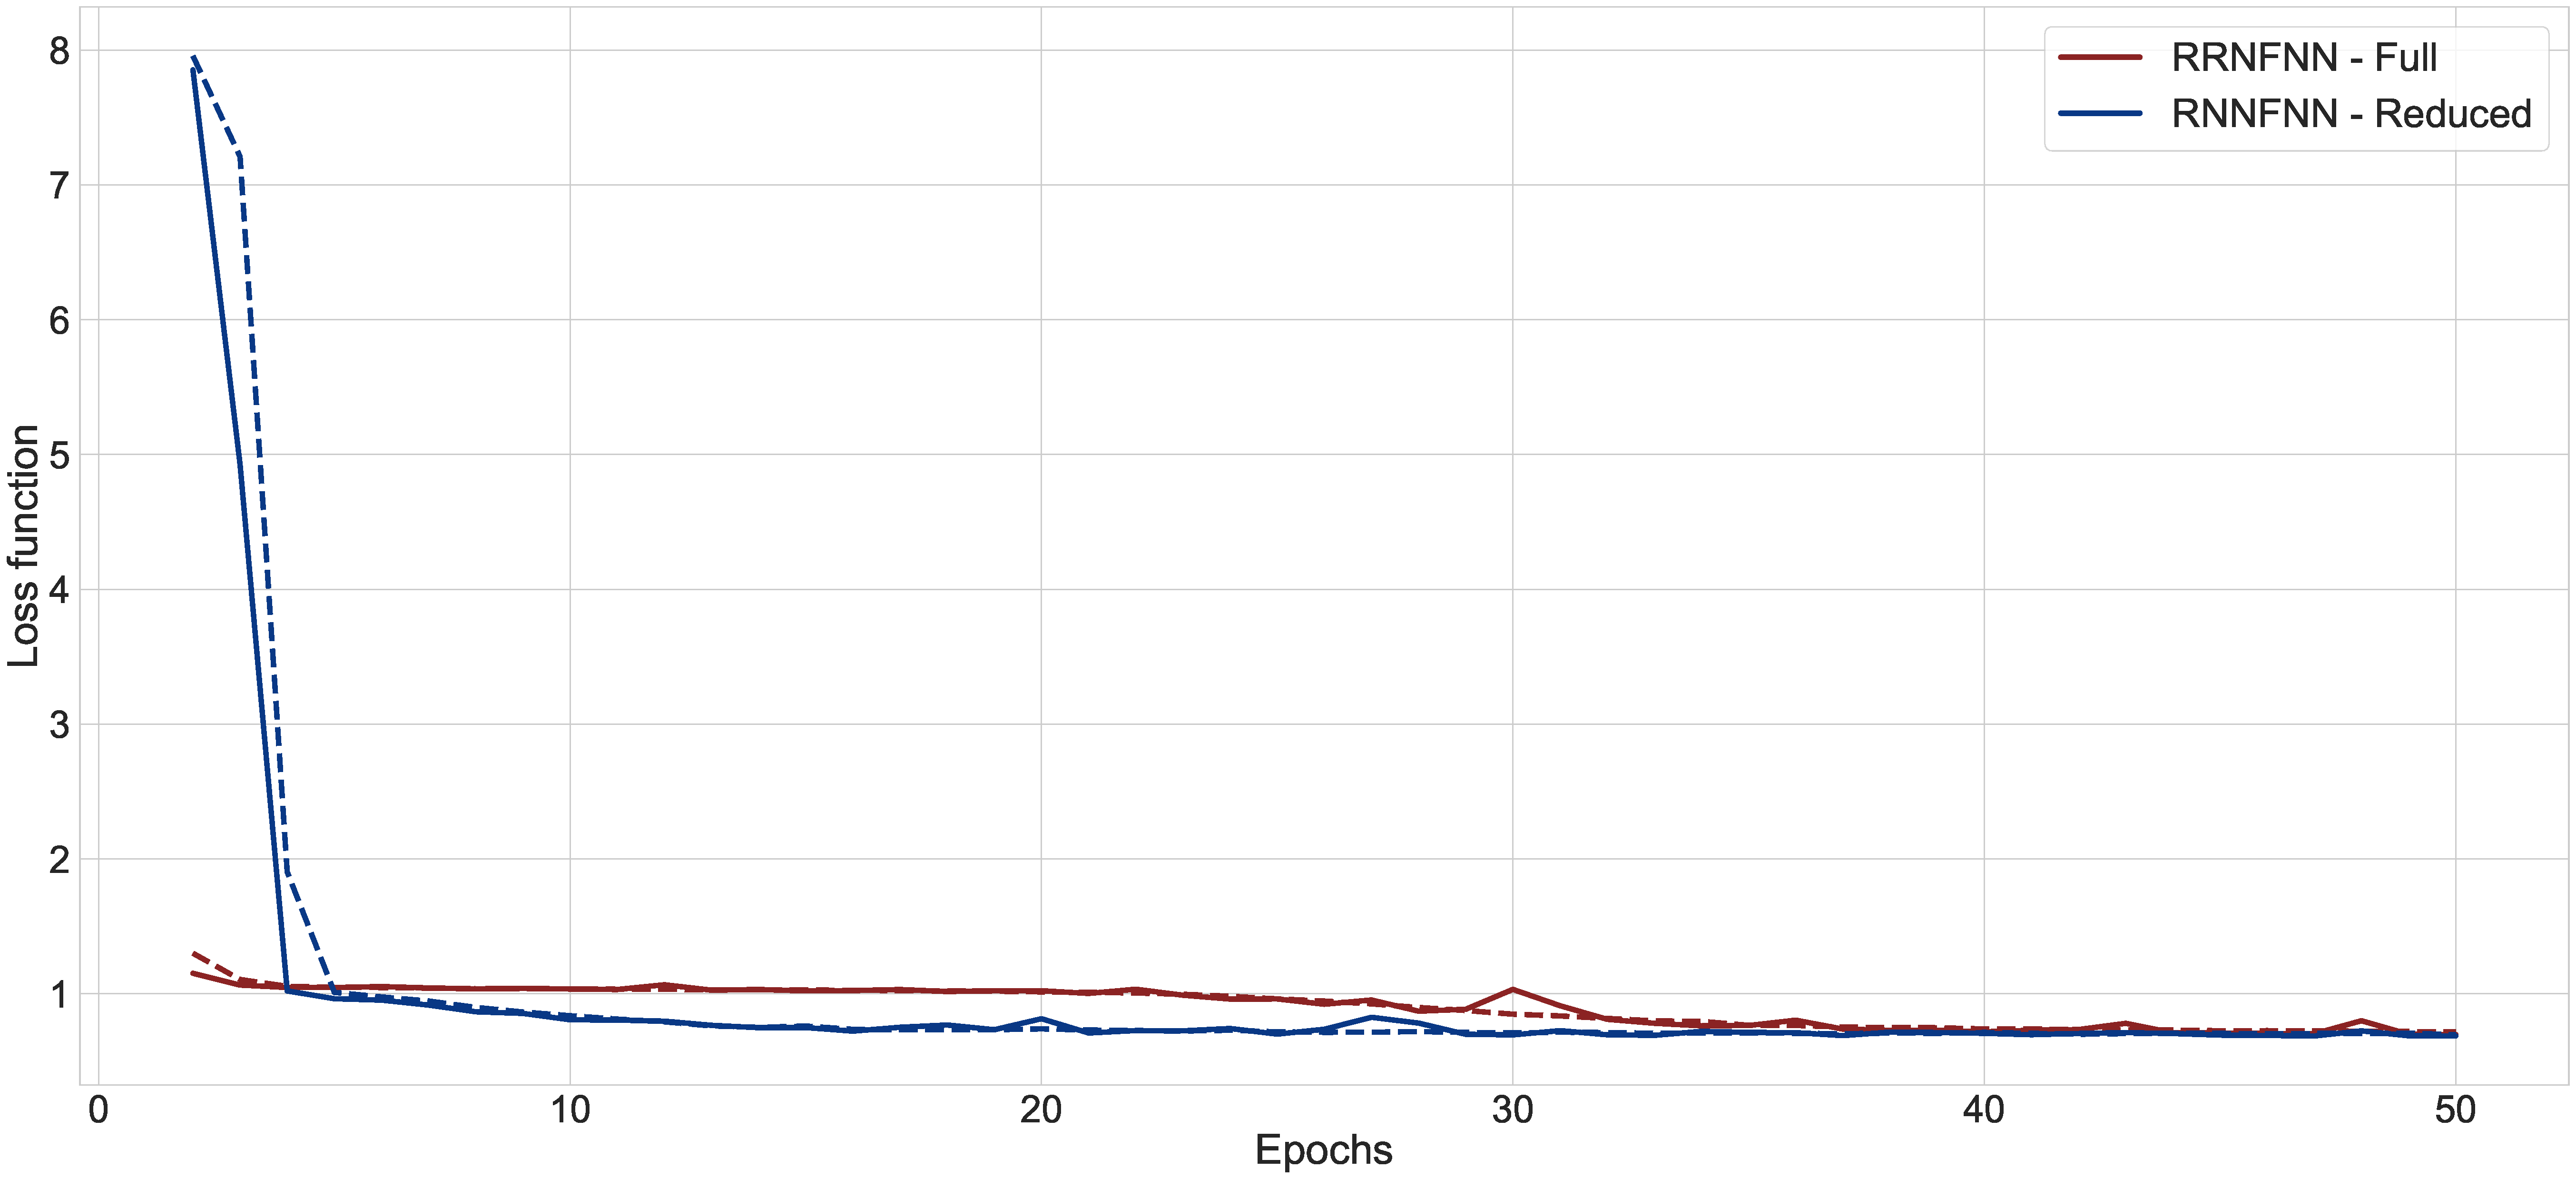
\includegraphics[width=16cm]{Plots/loss_curves_quadratic.pdf}
\begin{tablenotes}
\item \footnotesize Results are computed considering the MSE as the loss functions and the hedging error of 99,000 out-of-sample independent paths with random initialization for the validation loss curve (full line) and 400,000 independent paths fot the training loss curve (dash line). Simulations are performed based on the Black-Scholes model and agents are trained considering the cash constraint of $B=100$.
\end{tablenotes}
\label{fig:loss_curves_quadratic}
\end{figure}

Consistent with the findings detailed in Section \ref{subsub:state_space} regarding the dynamics of the JIVR model, the RL agent trained with the reduced state space exhibits improved the rate of convergence during the training phase. For instance, as depicted in \autoref{fig:loss_curves_quadratic}, the penalty curve evolution for the RL-MSE agent over 50 epochs illustrates this trend. This approach effectively reduces computational costs during training and accelerates convergence to optimal performance. These numerical outcomes confirm that our method achieves robust performance without necessitating the inclusion of portfolio value, even within the Quadratic Hedging framework with Black-Scholes market dynamics.

%\fredcomment{Maybe have a section related to \cite{horikawa2023relationship}, where we show the difference between the delta hedge and optimal does not look like a statistical arbitrage.}




\section{In-sample backtest}

In this section, we benchmark our approach using a historical path of the JIVR model spanning from January 5, 1996, to December 31, 2020, to assess the effectiveness of RL agents. This experiment examines their performance based on the historical series $\{R_{t},\beta_{t}\}$. Specifically, we evaluate the hedging performance considering a new European ATM call option with a maturity of 63 days every 21 business days along this historical path. The option prices, serving as initial hedging portfolio values, are determined with the prevailing IV surface on the day the hedge is initiated.

To assess the robustness of the model under more general market conditions, we conduct a comparison of cumulative P\&Ls, which are computed as the cumulative sums of the P\&L achieved by each strategy at the maturity of each option during the analyzed period. As illustrated in \autoref{fig:cumulative_p&l}, which depicts the evolution of the cumulative P\&L across two panels, each representing a different transaction cost level, the gap in cumulative P\&L between RL agents and benchmarks significantly widens as transaction cost rates increase. This, again, highlights the adaptability of the RL approach to various market conditions. 

\begin{figure}[H]\centering
\caption{Cumulative P\&L for ATM call options with a maturity of 63 days under real asset price dynamics.}
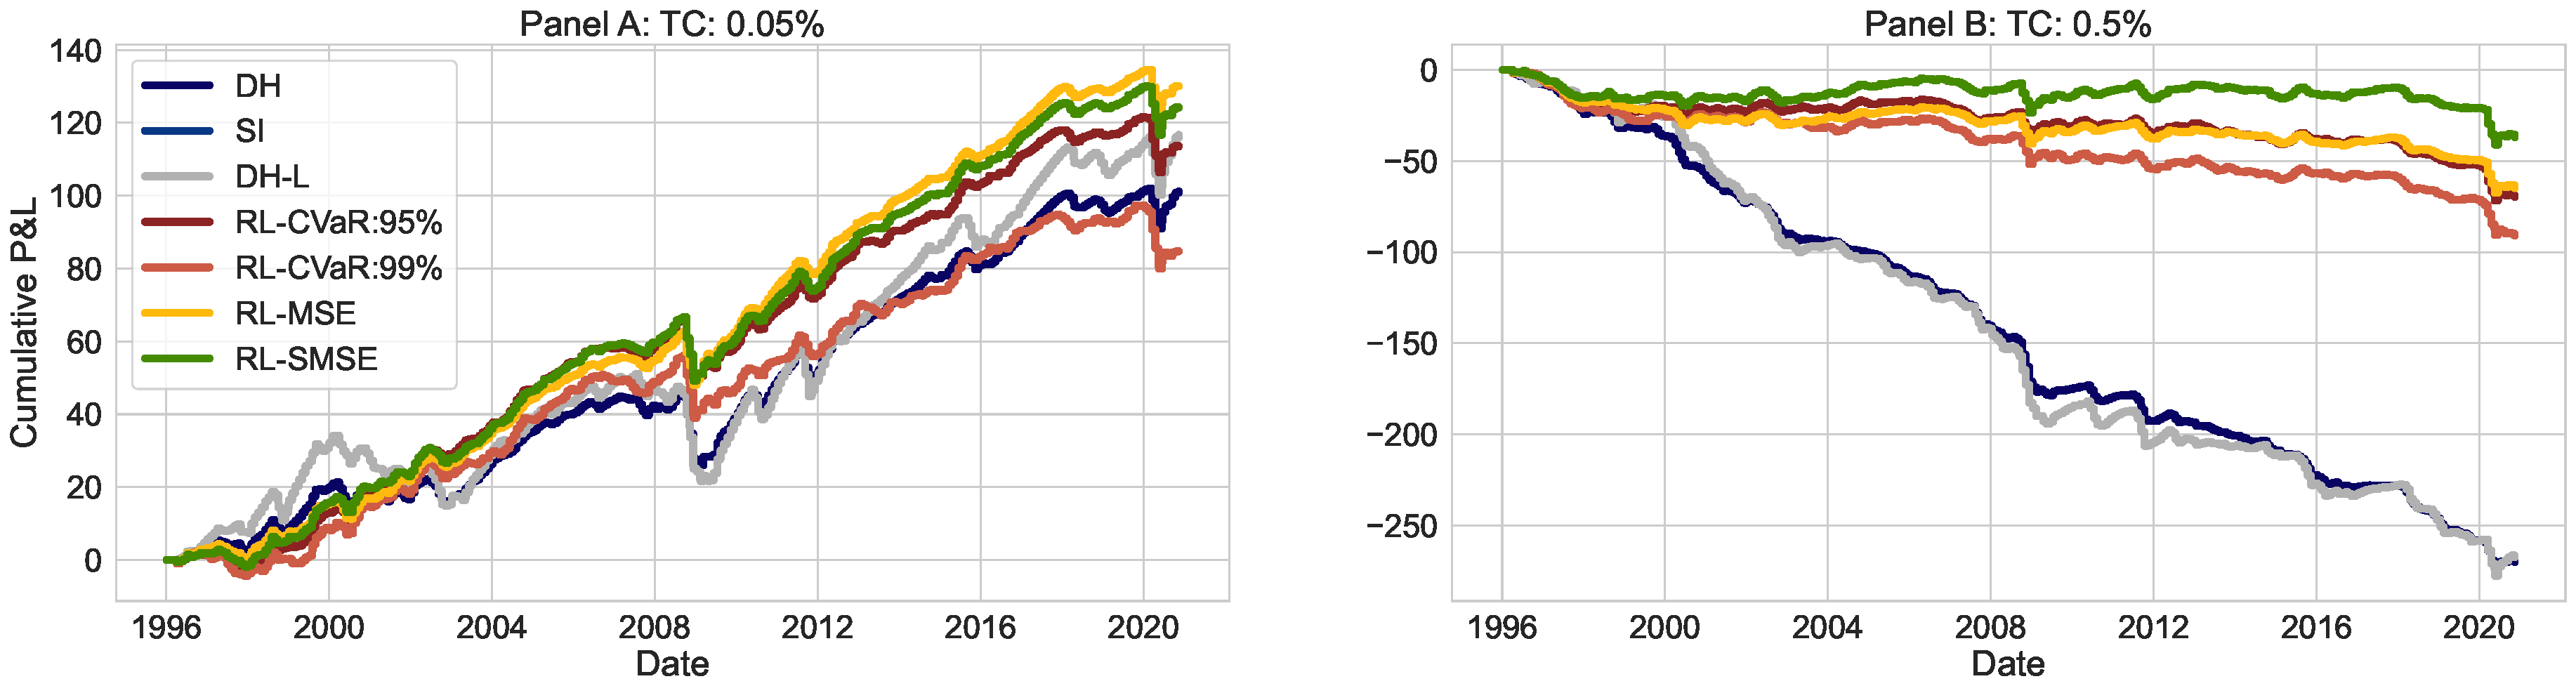
\includegraphics[width=17.5cm]{Plots/backtest_call_position.pdf}
\begin{tablenotes}
\item 
\footnotesize Results are computed based on the observed P\&L from hedging 296 simulated ATM Call options under real market conditions observed from May 1, 1996, to December 31, 2020. A new option is considered every 21 business days. Agents are trained under the reduced state space $(\delta_{t},\tau_{t},S_{t},\{\beta_{t,i} \}^5_{i=1}, h_{t,R})$ according to the conditions outlined in Section \ref{subsub:network_architecture}.
\end{tablenotes}
\label{fig:cumulative_p&l}
\end{figure}

In contrast to the findings presented in Section \ref{subsub:benchmarking_general}, where SI delta yielded the highest profitability among all strategies, the RL approach achieved the highest profitability in historical paths. Specifically, agents trained under the MSE and SMSE emerged as the most profitable ones.

Moreover, RL agents consistently outperform benchmarks across most of the transaction cost levels. However, when the transaction cost is small (left panel), Benchmarks exhibit a better cumulative P\&L compared to the RL agent trained under the CVaR$_{99\%}$ penalty function at the end of the period, December 31, 2020. Nevertheless, benchmarks also demonstrate more variability and larger losses, such as those observed between 2008 and 2012. In contrast, RL agents show a smaller decrease in cumulative P\&L, indicating more resilience during crisis periods. In general, the observed performance of the RL agents under historical data is consistent with our findings under simulated data, indicating the robustness of our approach.
